\section{Building Block View}

In this section we will describe the \gls{app} using some elements of the 4+1 Architectural View Model. With this model we will represent
the \gls{app} using five different views, which should focus on specific elements of the project. Each view provide
a different purpose \cite{refart:KR41}. For this project we will provide the 3 following views of the 4+1 Architectural View 
Model:

\begin{itemize}
    \item \textbf{Scenario view}: simple description for the end user 
    \item \textbf{Behaviour view}: description of the existing processes
    \item \textbf{Structural view}: object-oriented decomposition
\end{itemize}

The scenario view was presented in the figure \ref{fig:preliminary_use_case} of this project.

\subsection{Behaviour view}
The following \gls{activity diagram} depicts the register and login procedure within the app.

\begin{figure}[H]
    \centering
    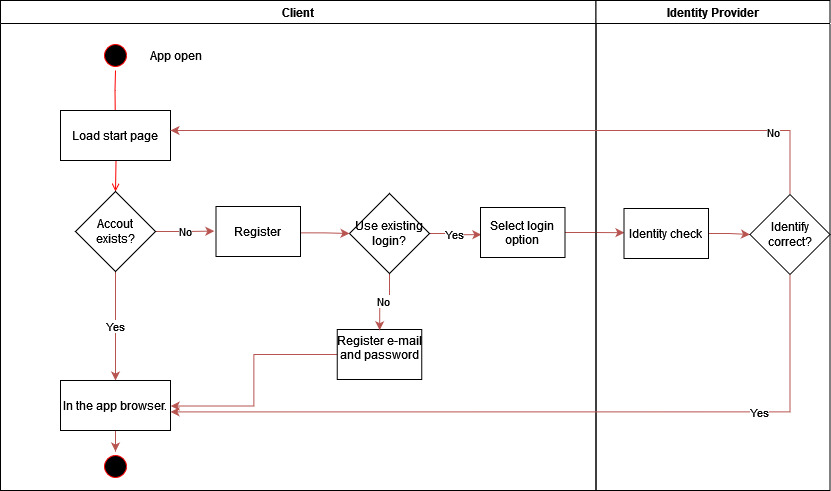
\includegraphics[width=1\textwidth]{assets/login_AC.jpg}
    \caption{Login procedures}
    \label{fig:login_register}
\end{figure}


\subsection{Structural view}
To describe this view we choose a \gls{class diagram}. With it we may provide a static description of elements
of our app. This will be very relevant for the developing process of the \gls{app}.

The first part of the this diagram describes the element within the \gls{provider}. It contains one or more addresses and it 
can offer one or more products. A provider will also fall into the category restaurant, bakery or pastry.

\begin{figure}[H]
    \centering
    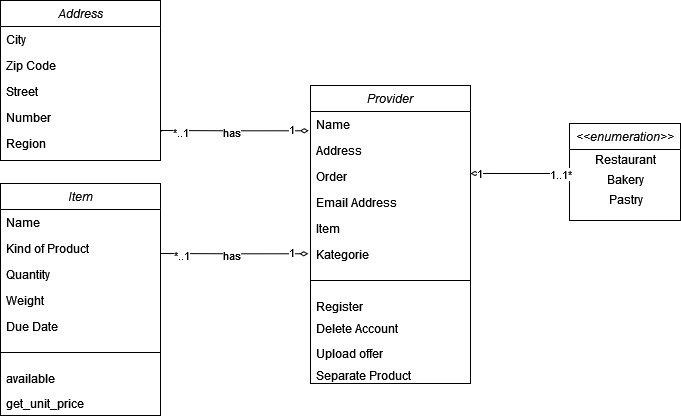
\includegraphics[width=0.6\textwidth]{assets/Provider_Addr_Item.jpg}
    \caption{Provider overview}
    \label{fig:Provider_addr_item}
\end{figure}
 
The class dedicated to the \glsplural{client} should be as simple as possible. It should provide basic interaction like
registering, logging, deleting account, viewing product and placing order. The two last actions will stablish the communication 
with the \glsplural{provider}.

\begin{figure}[H]
    \centering
    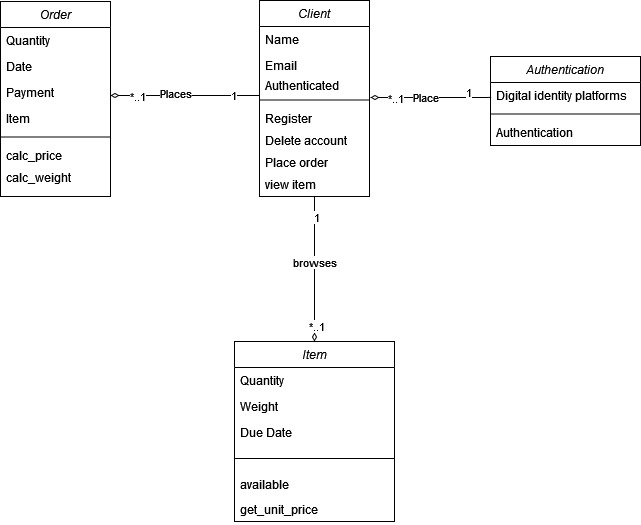
\includegraphics[width=0.6\textwidth]{assets/client_CD.jpg}
    \caption{Client Overview}
    \label{fig:client_CD}
\end{figure}

Finally we have an order placed by a \gls{client} and processed by a \gls{provider}. Here we will rely on a third party 
to stablish the payment procedures.

\begin{figure}[H]
    \centering
    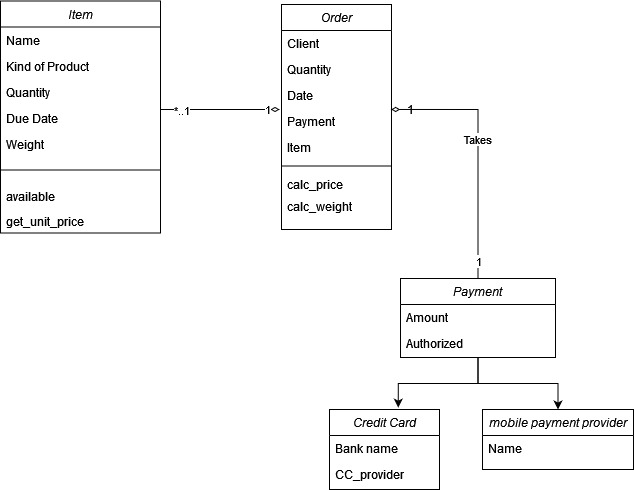
\includegraphics[width=0.6\textwidth]{assets/order_cd.jpg}
    \caption{Order Overview}
    \label{fig:order_cd}
\end{figure}

\newpage
\thispagestyle{lscape}
\begin{landscape}

This final graphic show the whole classes in combination:

\begin{figure}[H]
    \centering
    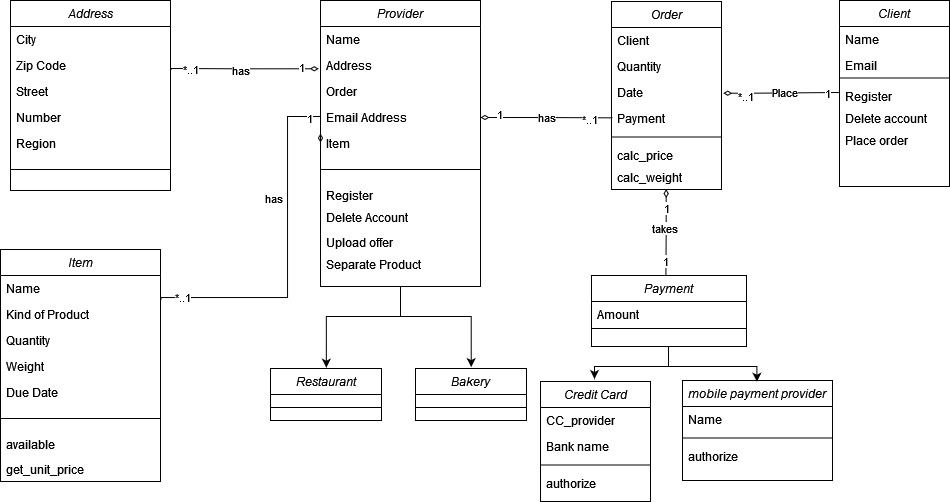
\includegraphics[width=1.5\textwidth]{assets/classes_CD.jpg}
    \caption{Classes Overview}
    \label{fig:class_CD}
\end{figure}

\end{landscape}
